\documentclass[11pt]{article}

% Use the following to compile
% mkdir tmp
% pdflatex -aux-directory=tmp -output-directory=tmp --shell-escape notes.tex

% Package use definitions
\usepackage[margin=1in]{geometry}
\usepackage{fancyhdr}
\usepackage[parfill]{parskip}
\usepackage{graphicx}
\usepackage{comment}
\usepackage[outputdir=tmp]{minted}
\usepackage[dvipsnames]{xcolor}
\usepackage{listings}
\usepackage[hidelinks]{hyperref}
\usepackage{amsmath}
\usepackage{amsfonts}
\usepackage{amssymb}
\usepackage{tcolorbox}
\usepackage{tabu}
\usepackage{upgreek}
\usepackage[ruled,vlined]{algorithm2e}
\usepackage[nottoc]{tocbibind}
\usepackage{natbib}
\usepackage{pdfpages}
\usepackage{pgffor}
\usepackage{minted}

\setlength{\parindent}{11pt}
\setlength{\parskip}{0pt}

% Header and footer setup
\pagestyle{fancy} \rhead{\today} \lhead{Enquette Budget Temps} \renewcommand{\headrulewidth}{1pt} \renewcommand{\footrulewidth}{1pt}

% Image directory specification
\graphicspath{ {./images/} }

% Settings minted option for the entire document
\definecolor{LightGray}{rgb}{0.9, 0.9, 0.9}
\setminted{frame=lines,framesep=2mm,linenos,
  fontsize=\footnotesize, baselinestretch=1.2}

% Start of document
\begin{document}

% Title page and table of contents setup
\begin{titlepage}
  \begin{center}
    \vspace*{1cm} \Huge \textbf{Enquette Budget Temps}\\
    \vspace*{1\baselineskip} Langage R et Analyse de donnée\\
    \vspace*{2\baselineskip} \large
    \vfill \normalsize \textbf{Etienne Sharpin}\\ \textbf{Jose
      A. Henriquez Roa}\\
    \vspace*{2\baselineskip} \today \rhead{\today}
    \newpage
    \normalsize \tableofcontents
    \newpage
  \end{center}
\end{titlepage}


\section{Description du jeu de données}

Ce jeu de données représente une enquête mettant en valeur le temps passé dans multiples activités au cours d’une journée (Budget/Temps).

La population étudiée provient de plusieurs pays différents et porte sur des hommes et des femmes de différentes situations.

\section{Chargement des données}

\begin{minted}{R}

path = "./Enquete_Budget_Temps.xlsx"
library("readxl")
df01 <- read_excel(path)

summary(df01)

\end{minted}

On charge les données depuis le fichier excel.

\section{Normalisation des distributions}

\begin{minted}{R}

df02 <- df01
df02[, 2:11] <- df01[, 2:11] / 2400

\end{minted}

On normalise les données en divisant chacune des valeurs numériques par 2400 ce qui nous permet une meilleur distribution afin d'obtenir de meilleurs résultats lors des différentes analyses statistiques que nous allons effectuer par la suite.

\newpage

\section{Analyse des boîtes à moustaches}
\begin{minted}{R}

df03 <- df02[2:11]

pdf("plot/box-plot.pdf")
boxplot(df03, use.cols=FALSE, las=2, ylab="Time percentage", main="Analytics of time spent per-activity")
dev.off()

\end{minted}

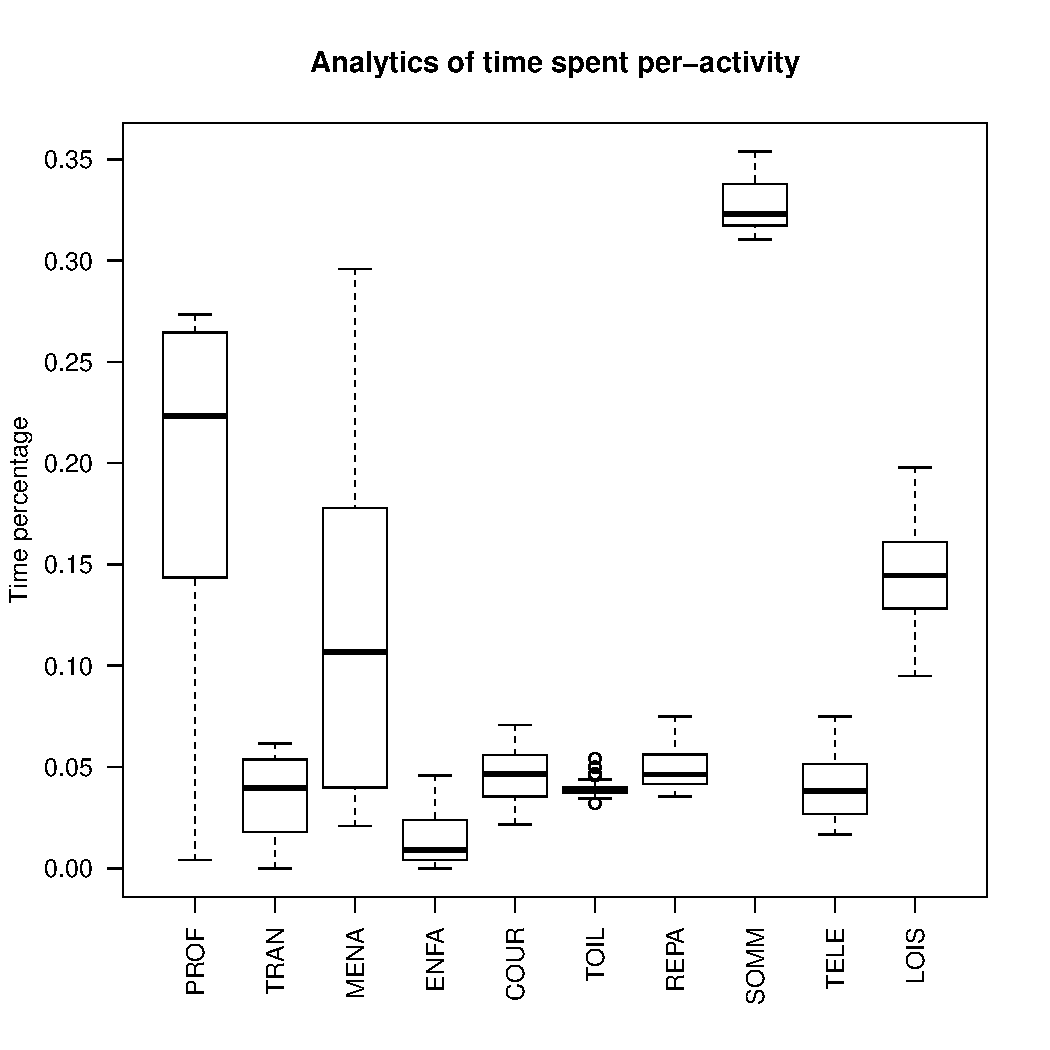
\includegraphics[scale=0.8]{../plot/box-plot.pdf}

Le diagramme en boîte à moustache est très utile notamment pour observer la dispersion des valeurs sur certaines variables. Ainsi, nous pouvons voir que certaines activités comme aller aux toilettes qui sont du ressort de la nécessité, sont une activité ayant très très peu de variance. Effectivement, chaque individus quelque soit sa classe a les mêmes besoins. On peut également l'observer au niveau du sommeil ou des repas, où l'écart est faible avec des valeurs relativements centrées.


Les valeures de certaines activitées sont bien plus dispersées, comme c'est le cas pour le travail ou le ménage et possède des temps bien plus conséquents que les autres activitées car étant considérées comme essentielles d'y consacrer du temps de vie.


\newpage

\section{Matrice de corrélation}

\begin{minted}{R}

pdf("plot/correlation-matirx.pdf")
library("PerformanceAnalytics")
chart.Correlation(df03, histogram=TRUE, title="hello")

mtext("Correlation Matrix", side=3, line=3)
dev.off()

\end{minted}


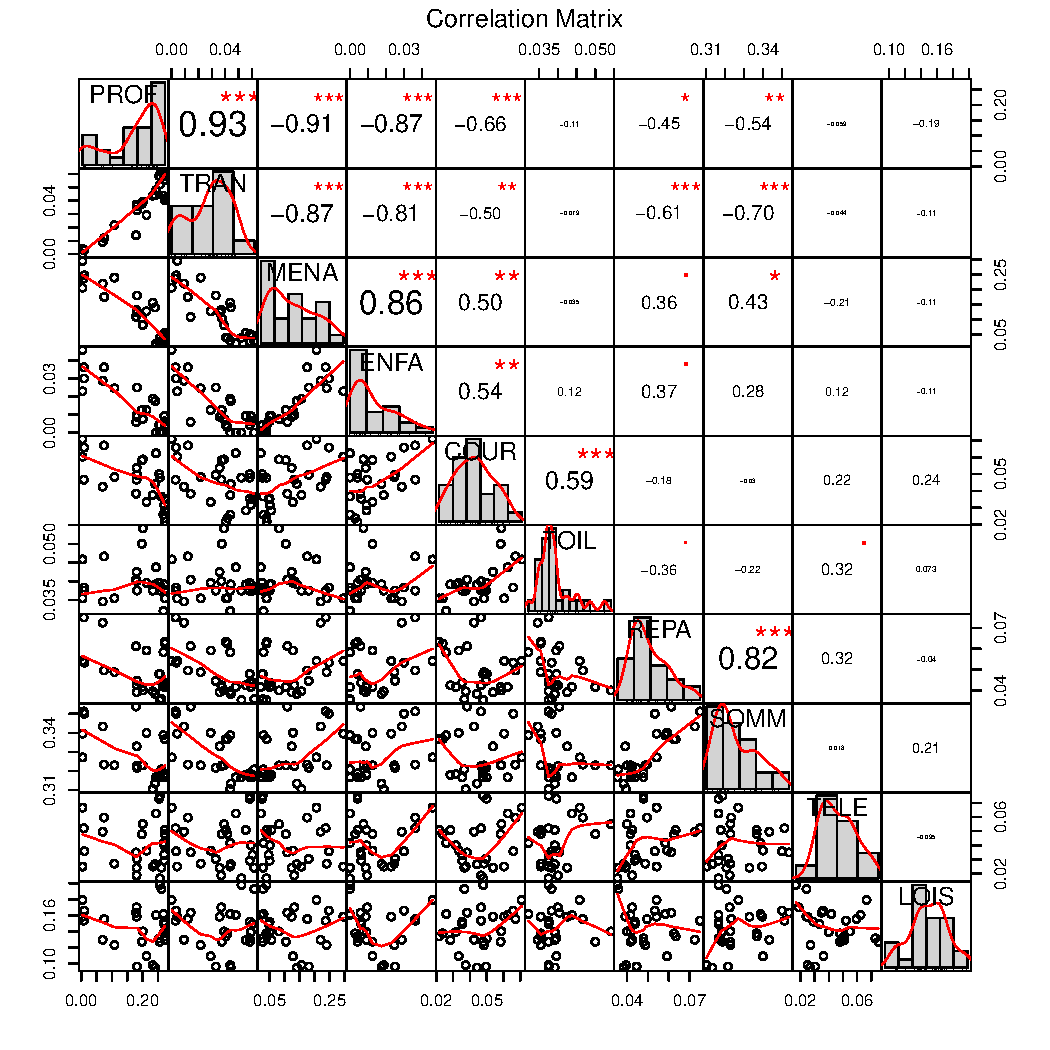
\includegraphics[scale=0.8]{../plot/correlation-matirx.pdf}


Cette matrice de corrélation met en évidence bon nombres de facteurs, typiquement, avec une corrélation casi linéaire positive de 0.93 entre le temps consacré au travail et celui passé dans les transports. En effet pour aller travailler il faut se déplacer. 

L'activité professionnelle étant très chronovore, elle est également en corrélation négative avec le ménage ou les enfants, en effet lorsque l'on est sur son lieu de travail, on est pas chez soi . Elle l'est d'ailleurs avec la plupart des autres activitées comme les activitées primaires même si elle influe également sur le temps de sommeil, en effet le travail pose des contraintes de sommeil plus stricts pouvant conduire les gens à moins dormir.

%% \section{Clustering}
%% \section{comparaison des profils}

\section{Carte Radar}
Pour comparer le temps alloué aux différentes tâches entre les individus de
différents groupes, nous avons choisi la méthode du graphique radar. Le code
suivant suivant montre comment nous avons tracé ces graphiques pour les 28
groupes, présentés dans l'annexe. Un graphique radar contenant tous les groupes
est présenté à la fin de cette section.
\begin{minted}{R}
library(fmsb)

pdf("plot/radar-chart-all.pdf")
df04 <- rbind(rep(max(df03),28), rep(min(df03),28), df03)
radarchart(df04, title="Per-Instance comparison")
dev.off()

for (i in 1:28) {
    pdf(paste("plot/radar-chart/radar-chart-", tolower(df01$ID[i]), ".pdf", sep=""))
    df05 <- rbind(rep(max(df03),28), rep(min(df03),28), df03[i,])
    radarchart(df05, title=df01$ID[i])
    dev.off()
}
\end{minted}
For this we have used the library \textit{fmsb} which includes the function
\textit{radarchart(...)} from which the plots were drawn. Figure
\ref{fig:radar-chart-all} shows a comparison of time distributions between all
groups present in the dataset. The individual radar charts can be found in the
annex \ref{section:annex}.
\begin{figure}[h]
  \centering
  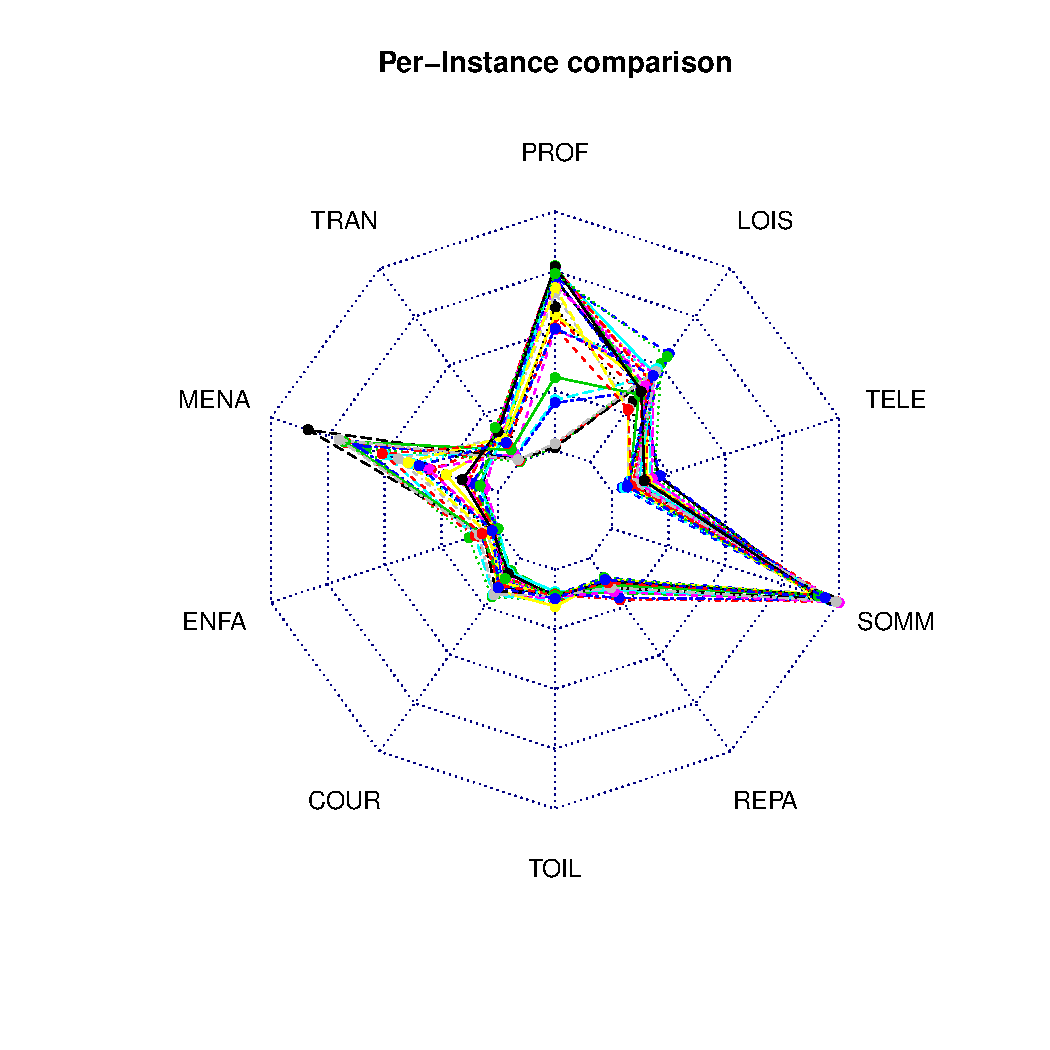
\includegraphics[scale=0.4]{../plot/radar-chart-all.pdf}
  \caption{Comparaison entre tous les groupes de profils}
  \label{fig:radar-chart-all}
\end{figure}

\newpage

\section{Graphique à barres}
Étant donné que les graphiques radar qui intègrent des valeurs de référence ont
tendance à avoir une allure plutôt encombrée, nous avons également choisi de
visualiser la distribution du temps à l'aide de diagrammes à barres, dans
lesquels nous avons inclus les pourcentages de temps sur l'axe des ordonnées.
\begin{minted}{R}
for (i in 1:28) {
    pdf(paste("plot/bar-plot/bar-plot-", tolower(df01$ID[i]), ".pdf", sep=""))
    barplot(t(as.matrix(df03[i,])), beside=TRUE, main=df01$ID[i],
            ylab="Time percentage", names.arg=colnames(df03), las=2)
    dev.off()
}
\end{minted}
Les graphiques générés sont dans l'annexe \ref{section:annex}
\section{ACP}
La ligne suivante effectue l'ACP que nous utilisons dans la section suivante de
clustering pour la visualisation des résultats.
\begin{minted}{R}
  pca = prcomp(df03)
\end{minted}
Les pourcentages de la variance expliquée pour chaque composante principale sont
obtenus par la commande suivante.
\begin{minted}{R}
  summary(pca)$importance[2,]
\end{minted}
qui produit le résultat suivant:\\\\ \texttt{PC1:\ 0.8804 PC2:\ 0.07166
  PC3:\ 0.02654 PC4:\ 0.01521 PC5:\ 0.0032 PC6:\ 0.00158 \\PC7:\ 0.00072
  PC8:\ 0.00043 PC9:\ 0.00026 PC10:\ 0}\\\\  Comme on peut le voir un peu plus
que 95\% de la variance est expliquée par les deux premières composantes
principales. Ce qui signifie que la projection bidimensionnelle des données sera
d'assez bonne qualité. Le graphique suivant est une représentation graphique de
la sortie ci-dessus.
\begin{minted}{R}
pdf("plot/principal-component-explained-variance.pdf")
barplot(summary(pca)$importance[2,],ylab="Explained Variance Proportion",
        ylim=c(0,1), main="Principal Component Explained Variance")
dev.off()   
\end{minted}
Le graphique résultant peut être vu dans la figure
\ref{fig:principal-component-explained-variance}.\par
\begin{figure}[H]
  \centering
  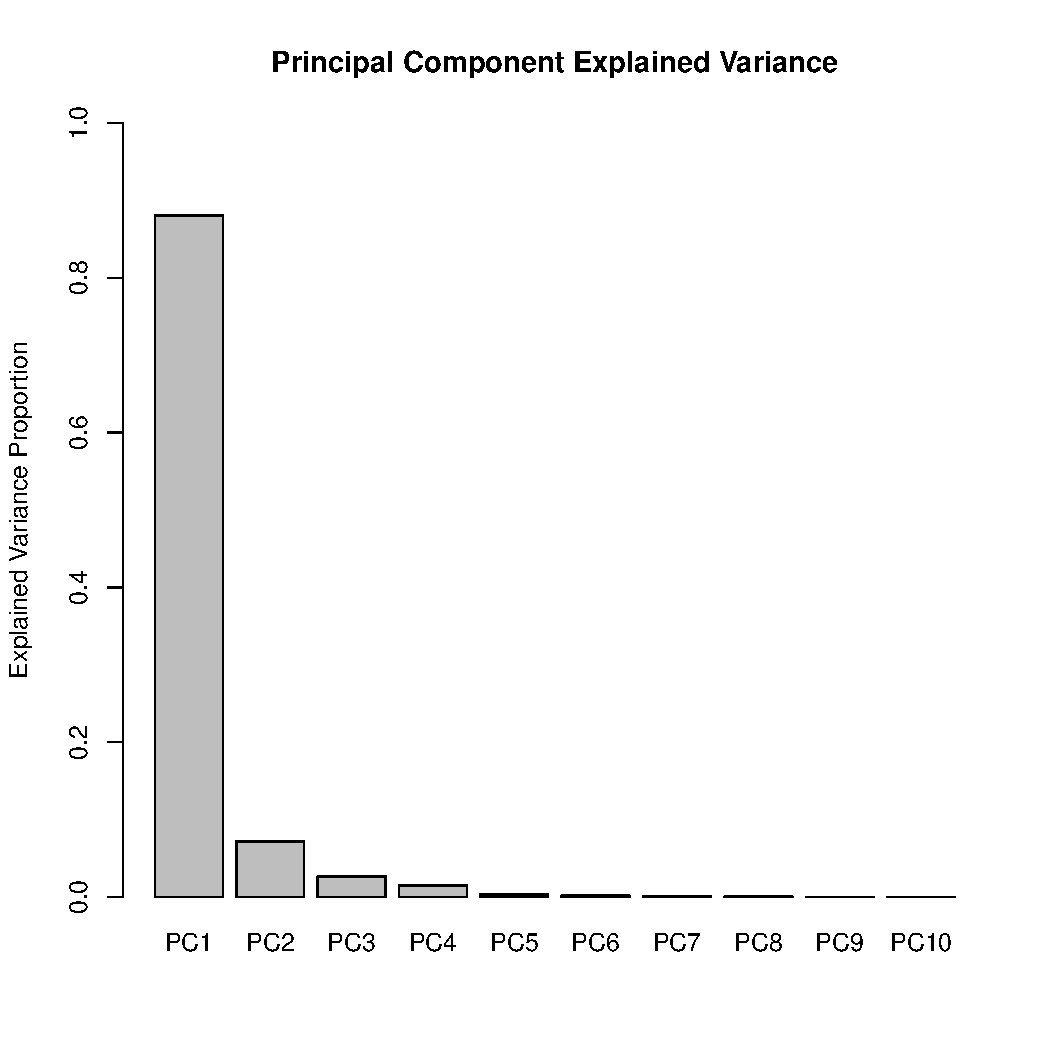
\includegraphics[scale=0.4]{../plot/principal-component-explained-variance.pdf}
  \caption{Principal component explained variance}
  \label{fig:principal-component-explained-variance}
\end{figure}
L'extrait de code suivant montre la projection de tous les attributs dans les
deux premières composantes principales.
\begin{minted}{R}
pdf("plot/pca-attribute-projection.pdf")
library("factoextra")
fviz_pca_var(pca, col.var = "cos2", col.ind = "cos2",
             gradient.cols = c("#00AFBB", "#E7B800", "#FC4E07"))
dev.off()
\end{minted}
Comme le montre la figure \ref{fig:pca-projection}. Dans celle-ci,
nous voyons que les deux attributs les mieux projetés sont de loin les attributs
PROF et MENA, correspondant respectivement aux attributs désignant le temps
passé à travailler et de nettoyage.\par Puis, la visualisation de la projection de
l'instance a été réalisée à travers le code suivant.
\begin{minted}{R}
pdf("plot/pca-instance-projection.pdf")
library("factoextra")
fviz_pca_ind(pca, col.var = "cos2", col.ind = "cos2",
             gradient.cols = c("#00AFBB", "#E7B800", "#FC4E07"))
dev.off()  
\end{minted}
Le graphique résultant est dans la figure \ref{fig:pca-projection}.
\begin{figure}[H]
  \centering
  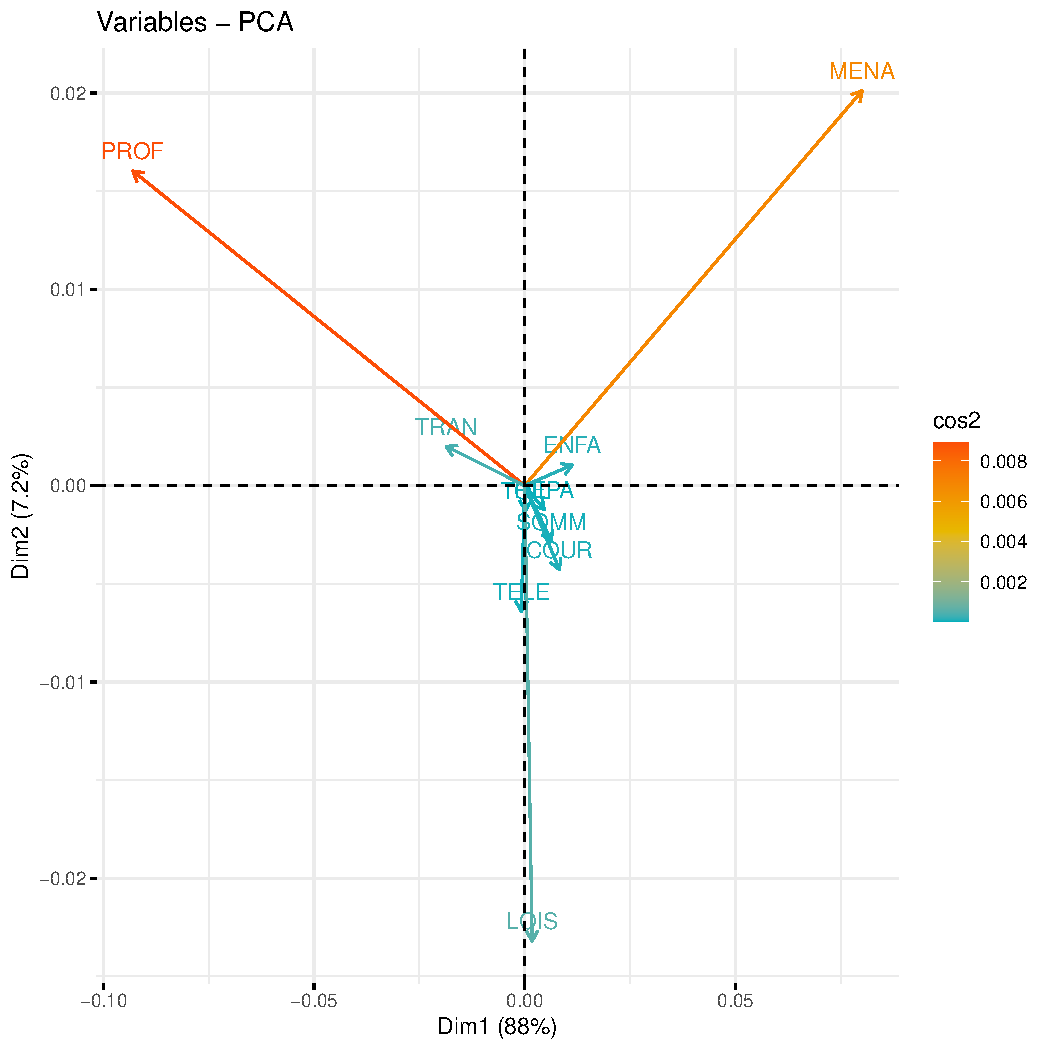
\includegraphics[scale=0.4]{../plot/pca-attribute-projection.pdf}
  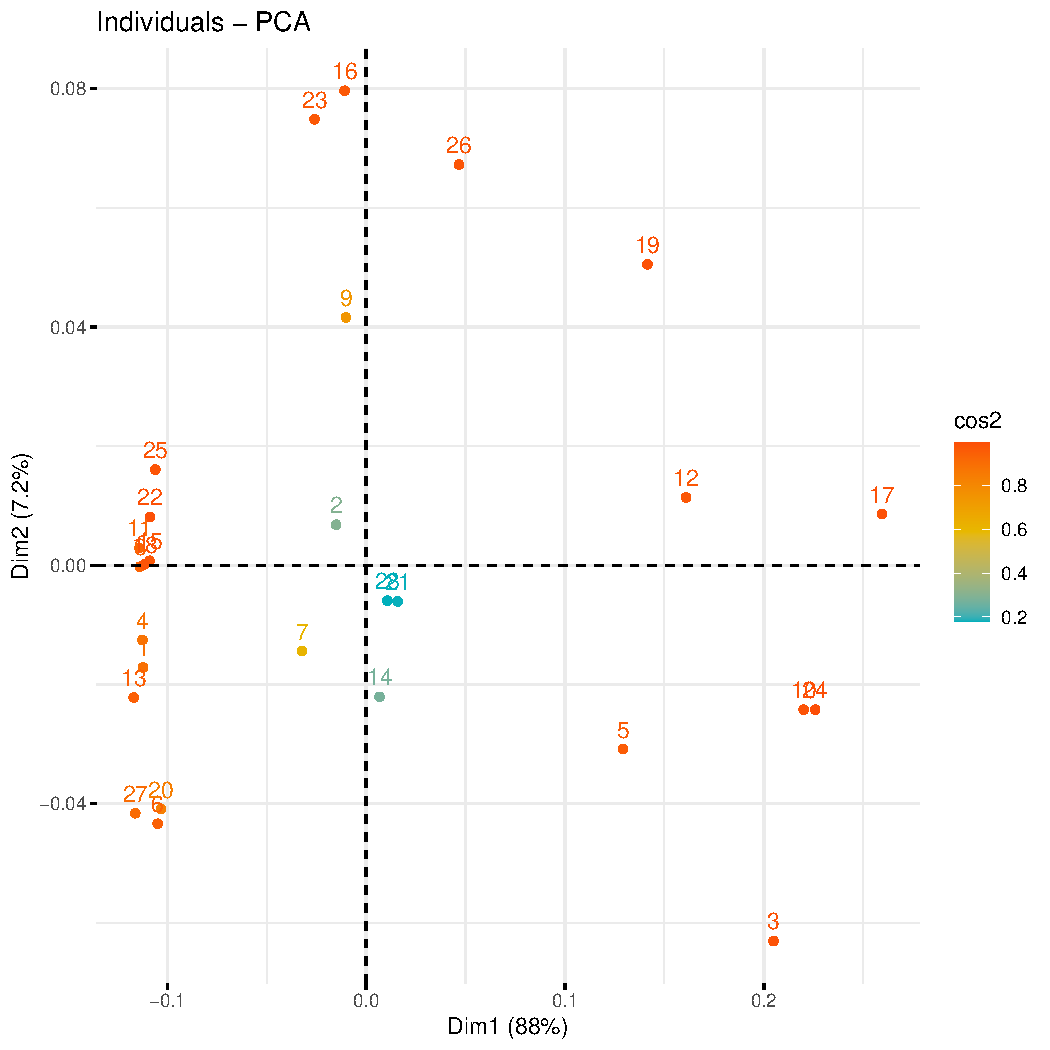
\includegraphics[scale=0.4]{../plot/pca-instance-projection.pdf}
  \caption{projection d'attributs (à gauche) et projection d'instances (à droite)}
  \label{fig:pca-projection}
\end{figure}
D'après les pourcentages de variance expliquée, nous constatons que la plupart
des instances ont une bonne qualité de projection.
\section{Clustering}
Pour analyser les similitudes entre les profils, nous avons regroupé les
instances à l'aide de l'algorithme d'apprentissage automatique KMeans. Cet
algorithme nécessite d'abord de définir manuellement le nombre de clusters dans
lesquels les instances seront regroupées. Ceci est fait dans le code suivant.
\begin{minted}{R}
pdf("plot/kmeans-inertia.pdf")
fviz_nbclust(df03, kmeans, method="wss")
dev.off()
pdf("plot/kmeans-silhouette.pdf")
fviz_nbclust(df03, kmeans, method="silhouette")
dev.off()
pdf("plot/kmeans-gap-stat.pdf")
fviz_nbclust(df03, kmeans, method="gap_stat")
dev.off()  
\end{minted}
Les trois graphiques sont présentés dans la figure \ref{fig:cluster-count}. Dans
ceux-ci, la courbe de score Silhouette et la statistique d'écart montrent que
deux sont une bonne quantité de clusters. Alors que la courbe du coude montre
également que trois est une bonne option. Ainsi, en prenant tous les résultats
en compte, nous avons choisi deux clusters pour les suivants analytique.\par
\begin{figure}[h]
  \centering
  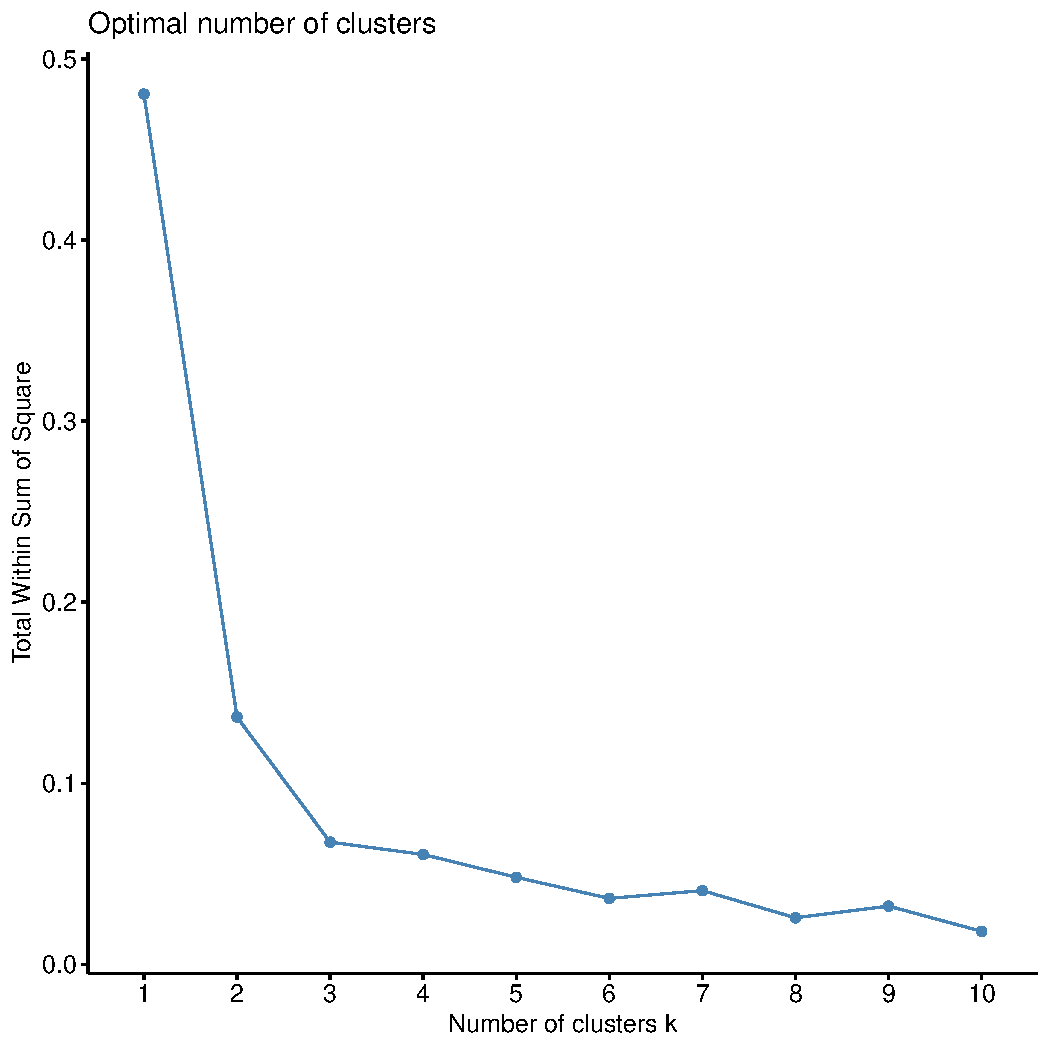
\includegraphics[scale=0.3]{../plot/kmeans-inertia.pdf}
  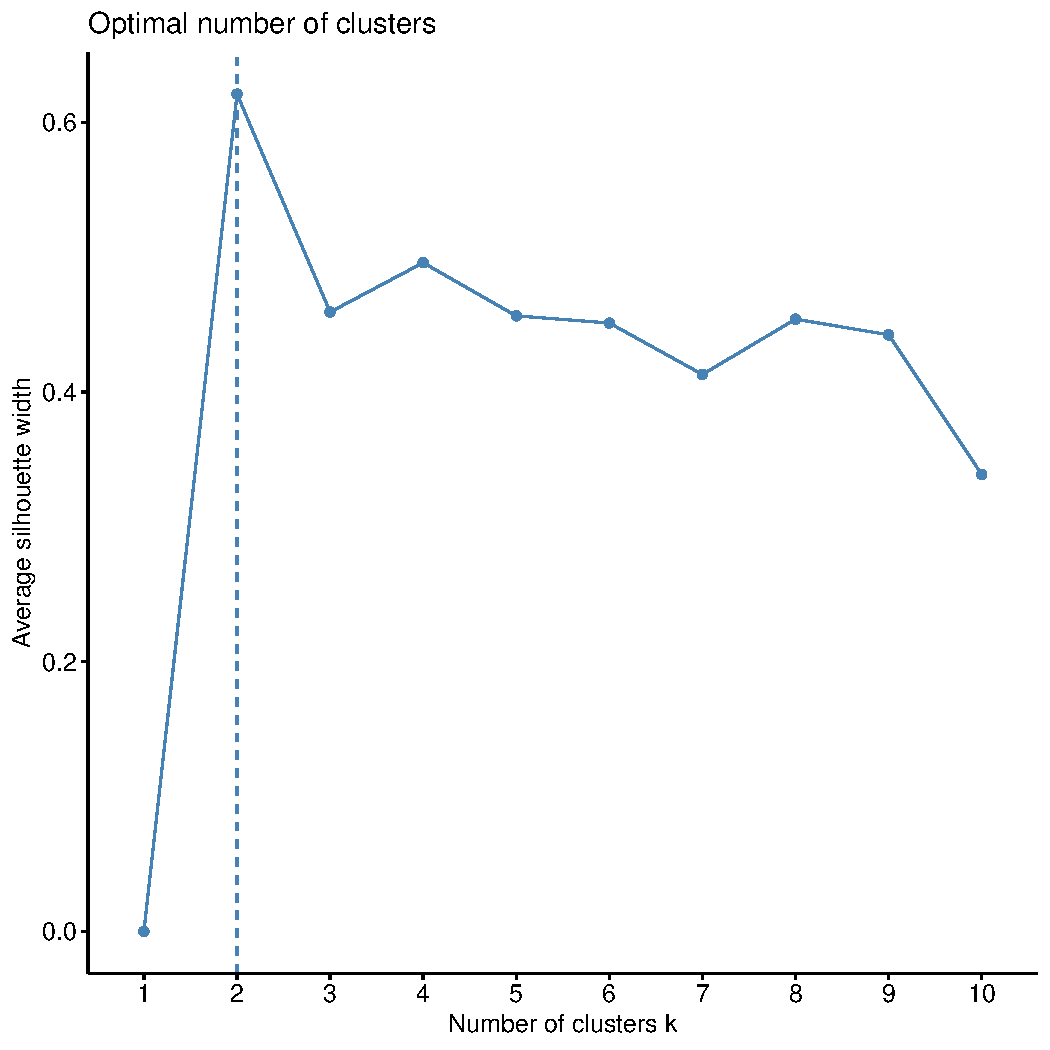
\includegraphics[scale=0.3]{../plot/kmeans-silhouette.pdf}
  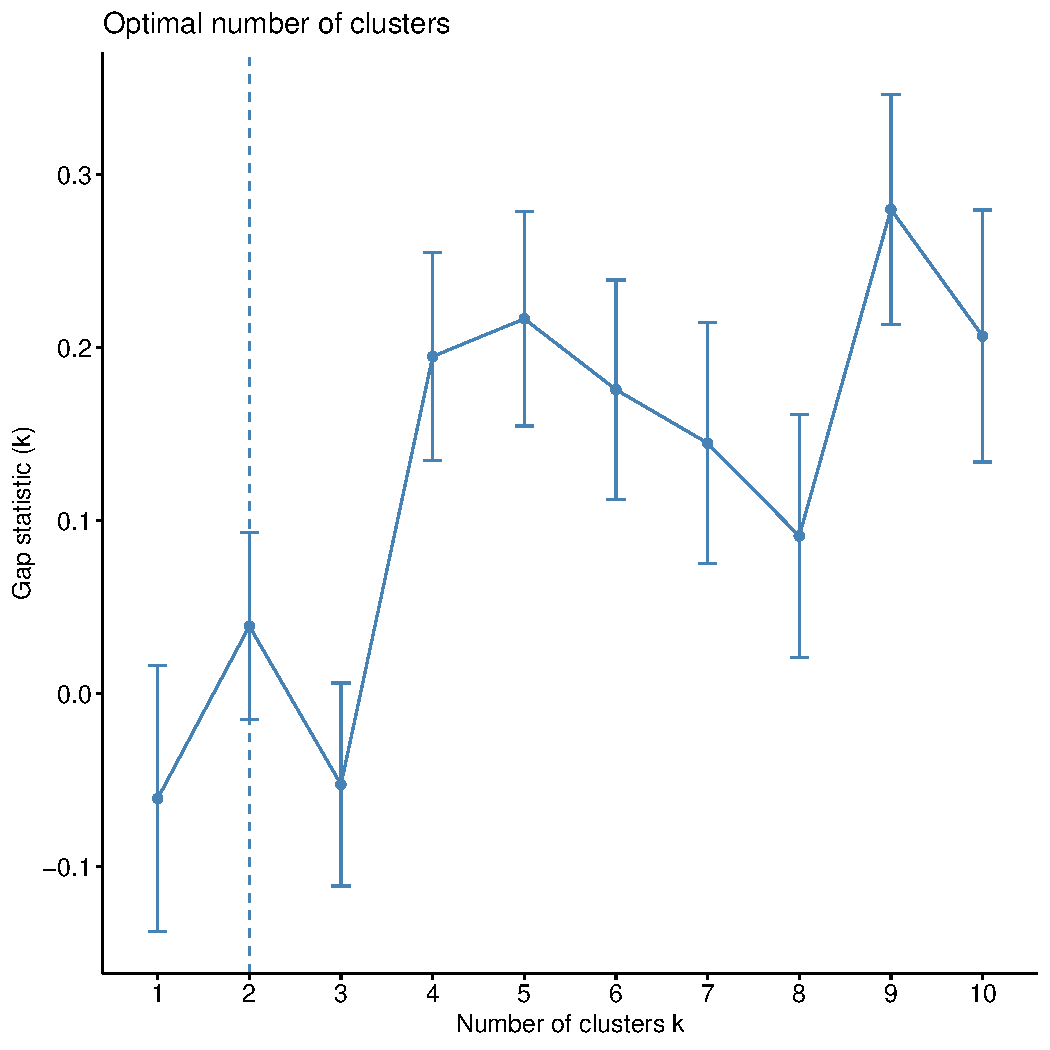
\includegraphics[scale=0.3]{../plot/kmeans-gap-stat.pdf}
  \caption{Courbe du coude (droite), scores de la silhouette (centre), statistiques de l'écart (droite)}
  \label{fig:cluster-count}
\end{figure}
Enfin, le clustering lui-même a été effectué avec l'extrait de code suivant.
\begin{minted}{R}
pdf("plot/clusters.pdf")
km = kmeans(df03, centers=2, nstart=25)
fviz_cluster(km, data=df03)
dev.off()
\end{minted}
Le résultat est dans la figure \ref{fig:clusters}.
\begin{figure}[h]
  \centering
  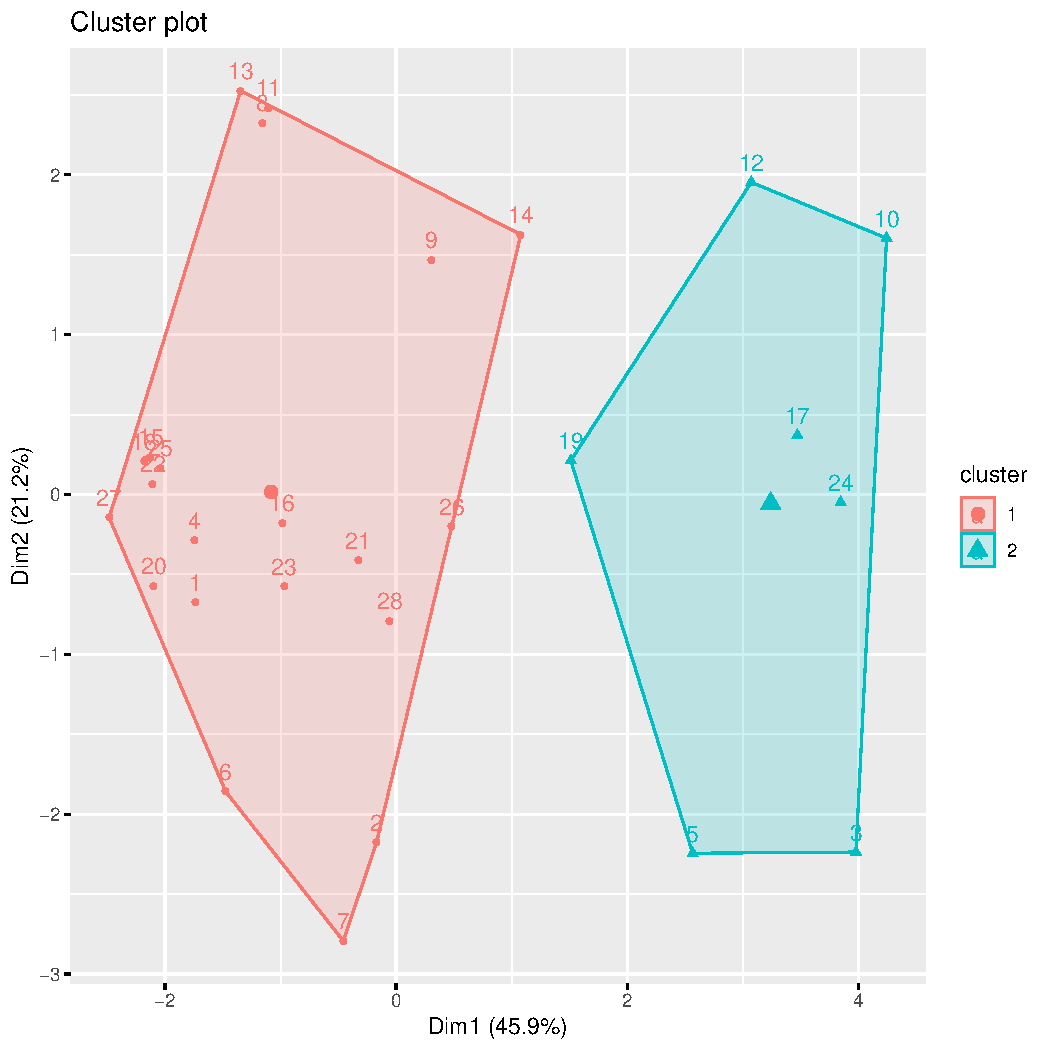
\includegraphics[scale=0.4]{../plot/clusters.pdf}
  \caption{Clustering}
  \label{fig:clusters}
\end{figure}
Pour le nombre d'instances par cluster, nous avons.
\begin{minted}{R}
print(paste("cluster01:", nrow(df01[km$cluster==1,])))
print(paste("cluster02:", nrow(df01[km$cluster==2,])))
\end{minted}
ce qui donne le résultat suivant:\\\\
\texttt{[1] "cluster01: 21"}\\
\texttt{[1] "cluster02: 7"}\\\\
Nous constatons qu'il n'y a pas un nombre uniforme d'instances par groupe, ce
qui signifie que l'algorithme ML a travaillé sur un certain type d'intuition
obtenue à partir des données lors du regroupement.\par Ensuite, pour voir à quel
point les instances d'un même cluster sont réellement similaires, nous
échantillonnons deux instances de clusters différents puis deux instances du
même cluster et nous les comparons. La figure suivante montre d'abord la
comparaison entre deux instances de clusters différents, puis la comparaison de
deux instances du même cluster.\par
\begin{minted}{R}
pdf("plot/fne-hme-comparison.pdf")
instanceIndices = c(24,25)
df04 <- rbind(rep(max(df03),28), rep(min(df03),28), df03[instanceIndices,])
title = paste(df01$ID[instanceIndices[1]],"-",df01$ID[instanceIndices[2]],
              "Comparison", sep=" ")
radarchart(df04, title=title)
dev.off()
pdf("plot/hme-fay-comparison.pdf")
instanceIndices = c(25,16)
df04 <- rbind(rep(max(df03),28), rep(min(df03),28), df03[instanceIndices,])
title = paste(df01$ID[instanceIndices[1]],"-",df01$ID[instanceIndices[2]],
              "Comparison", sep=" ")
radarchart(df04, title=title)
dev.off()
\end{minted}
Le résultat est dans la figure \ref{fig:fne-hme-comparison}.\par
\begin{figure}[h]
  \centering
  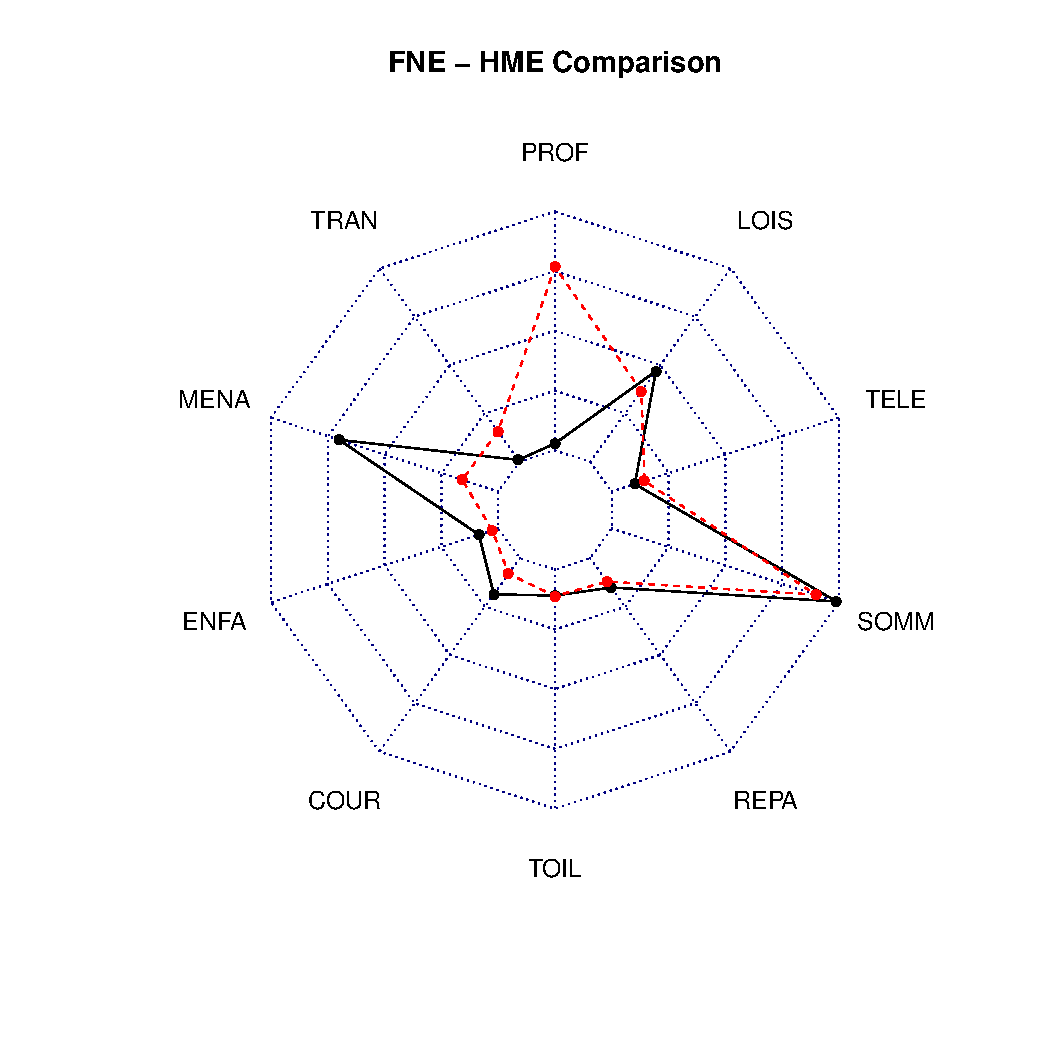
\includegraphics[scale=0.4]{../plot/fne-hme-comparison.pdf}
  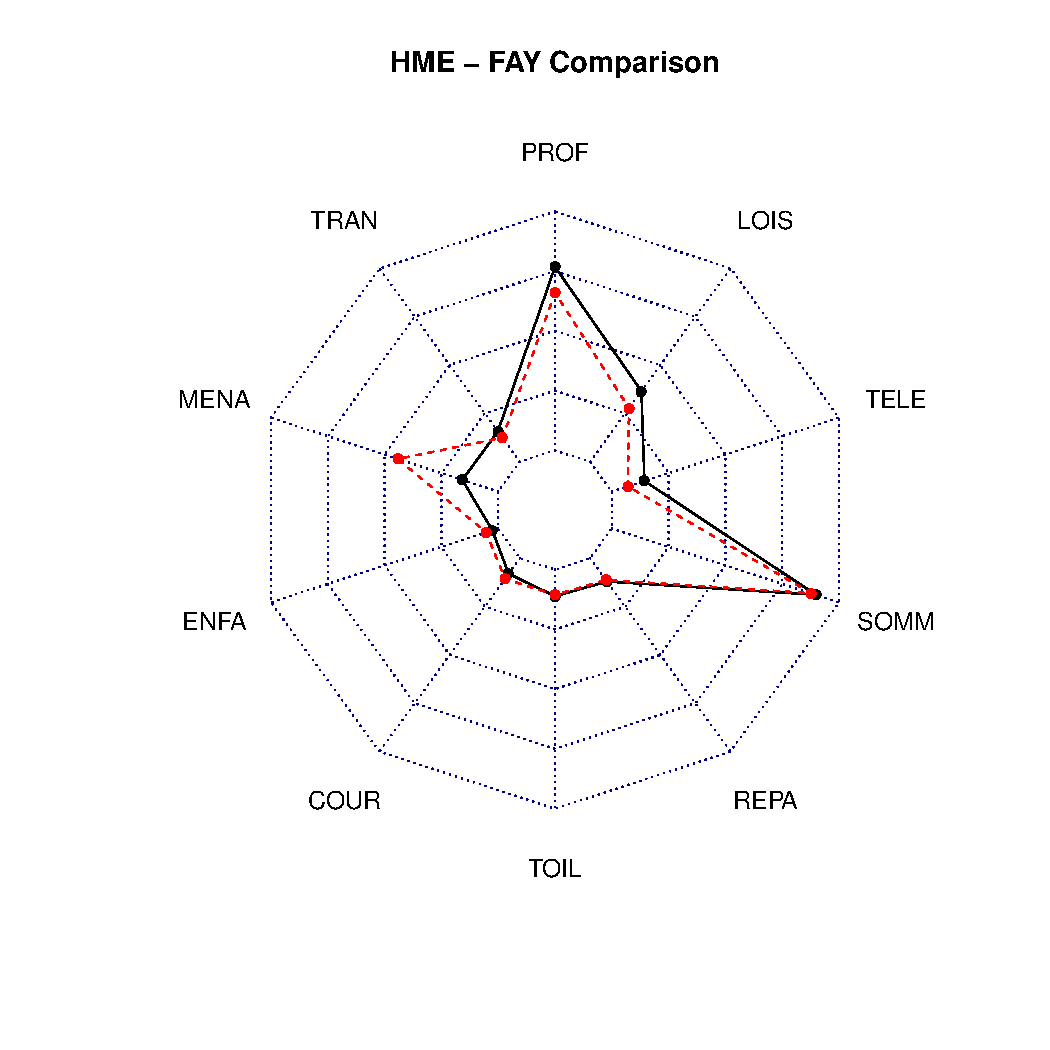
\includegraphics[scale=0.4]{../plot/hme-fay-comparison.pdf}
  \caption{Comparaison par cluster}
  \label{fig:fne-hme-comparison}
\end{figure}
Dans le graphique de gauche, nous voyons qu'entre ces deux cas, il y a une
différence considérable entre le temps passé à nettoyer et à travailler. Alors
que le cas le plus à droite est assez similaire tout du long.
\section{Critiques}
La principale critique à laquelle je peux penser est liée au fait que les
données ont déjà été traitées et que les individus ont déjà été regroupés comme
indiqué dans la description des données. Ce qui nous laisse avec la seule option
de faire une analyse secondaire, contenant tous les possibles biais de l'analyse
précédente.
\section{Annex}
\label{section:annex}
\subsection{Carte Radar}
\foreach\x in {1, ..., 28}{%
  \includegraphics[height=5.4cm]{../plot/radar-chart/radar-chart-\x.pdf}
}
\subsection{Graphique à barres}
\foreach\x in {1, ..., 28}{%
  \includegraphics[height=5.4cm]{../plot/bar-plot/bar-plot-\x.pdf}
}
\end{document}
